\documentclass{uai2021} % for initial submission
% \documentclass[accepted]{uai2021} % after acceptance, for a revised
                                    % version; also before submission to
                                    % see how the non-anonymous paper
                                    % would look like
%% There is a class option to choose the math font
% \documentclass[mathfont=cm]{uai2021} % Computer Modern math instead of
                                       % ptmx, like default for UAI ≤2020
% \documentclass[mathfont=newtx]{uai2021} % newtx fonts (improves upon
                                          % ptmx; less tested, no support)
% NOTE: Only keep *one* line above as appropriate, as it will be replaced
%       automatically for papers to be published. Do not make any other
%       change above this note for an accepted version.

%% Choose your variant of English; be consistent
\usepackage[american]{babel}
% \usepackage[british]{babel}

%% Some suggested packages, as needed:
\usepackage{natbib} % has a nice set of citation styles and commands
    \bibliographystyle{plainnat}
    \renewcommand{\bibsection}{\subsubsection*{References}}
\usepackage{mathtools} % amsmath with fixes and additions
\DeclarePairedDelimiterX{\infdivx}[2]{(}{)}{%
  #1\;\delimsize\|\;#2%
}
% \usepackage{siunitx} % for proper typesetting of numbers and units
\usepackage{booktabs} % commands to create good-looking tables
\usepackage{tikz}
\usepackage{graphicx} % nice language for creating drawings and diagrams

%% Provided macros
% \smaller: Because the class footnote size is essentially LaTeX's \small,
%           redefining \footnotesize, we provide the original \footnotesize
%           using this macro.
%           (Use only sparingly, e.g., in drawings, as it is quite small.)

%% Self-defined macros
\newcommand{\swap}[3][-]{#3#1#2} % just an example

\title{Image Classification using Unlabelled Data - A Semisupervised Approach using Variational Autoencoder and Topdown Hierarchical Clustering}

% The standard author block has changed for UAI 2021 to provide
% more space for long author lists and allow for complex affiliations
%
% All author information is authomatically removed by the class for the
% anonymous submission version of your paper, so you can already add your
% information below.
%
\author[1]{\href{mailto:Sunil Kumar Vengalil <sunilkumar.vengalil@iiitb.org> ?Subject=Your UAI 2021 paper}{Sunil Kumar Vengalil}{}}
\author[2]{Prathyush S.P}
\author[1]{Neelam Sinha}
% Add affiliations after the authors
\affil[1]{%
    International Institute of Information Technology Bangalore\\
}
\affil[2]{%
    Worcester Polytechnic Institute \\
   100 Institute Rd, Worcester, MA 01609, United States
}

\begin{document}
\maketitle

\begin{abstract}
The success of deep learning for solving complex tasks like image classification, segmentation, speech and natural language processing, has caused wide-spread interest in the machine learning community to focus on developing models and representations that are more explainable, and generalize better.
In this work, we propose an approach for using representations learned by unsupervised generative learning for solving tasks like image classification at a reduced manual annotation cost.
Our method is an alternate paradigm for supervised learning.
In existing supervised learning methods,  all samples are labelled prior to start of training whereas we propose an active learning mechanism where manual hints are given at regular intervals during training.
We demonstrate the proposed idea by training a  variational autoencoder on MNIST data set.
After every epoch of training, the low dimensional latent vectors are clustered and cluster centers are annotated.
The loss function in successive training is modified to incorporate the manual annotation.
In addition to achieving classification of digits, the approach also results in improved reconstruction accuracy and more regular features of autoencoder.
Our network architecture and cost function look similar to multi task learning with hard parameter sharing.
However, unlike other multi task learning models, our main goal is to reduce the manual annotation required for supervised tasks like image classification and segmentation.
The approach is demonstrated by classifying the images in MNIST data without using the label provided in the dataset.
We obtain a classification accuracy of 93.47\% on MNIST test images with 5 epochs of training.
\end{abstract}

\section{Introduction}\label{sec:intro}
Classifying images is one of the first use cases proven to give good results using deep neural networks.
Recently, there has been a lot of work on generative models like variational autoencoder(VAE)\cite{kingma2013auto} and generative adversarial network(GAN) \cite{goodfellow2014generative} on using deep neural network for learning distribution of high dimensional data.
In this work, we propose a method whereby a generative model like VAE can easily be converted into a classification model which is currently solved by a supervised classification method.
Note that the existing deep learning approaches for classification  need a lot of annotated training data and enormous training time on GPU\cite{krizhevsky2012imagenet}\cite{simonyan2014very}\cite{he2016deep}.
The approach proposed in this paper needs very less amount of manual annotation ( 10-16 samples in case of MNIST dataset)  and less computing resources.
We demonstrate our claim by building a classification model for MNIST dataset using all traning images in an unsupervised way and annotations are done only for selected representative samples.
The proposed approach augments a  variational autoencoder with a classification layer the loss component of which is tuned using manually annotated samples at regular training intervals.


A generative model learns the distribution of data $p(x_{ij})$.
A new image of a given digit can be generated by sampling from this distribution.
In the case of an image, this is usually a complex distribution in a high dimensional space of dimension $W \times H$.
Such a distribution in the original high dimensional space is not of much use as it is not easy to visualize and contains too many  minute details.
Specifically, the properties of interest, like line thickness in case of handwritten digit, are not explicitly evident from such a distribution.
All generative models essentially solve this problem by transforming the original image into a much low dimensional latent space, which we denote by  $Z$.
For each image $x^n \in X$, there exists a latent vector  $z^n \in Z$  where $z^n$ is of dimension $z_{dim}$.
The dimension of latent space $z_{dim}$ is much less compared to the original image dimension.
However, one of the major issues with these trained models is that the concepts represented by latent dimensions need not make any sense and hence they lack one of the much needed properties: the model explainability.


In this work, we propose an active learning framework using variational autoencoder for the task of  image classification.
Variational autoencoder is used for learning a low dimensional latent representation which is used for classification task.


Our model is similar to multi task learning since the loss term has both reconstruction and classification losses.
However, unlike most other multi-task models, see \cite{ruder2017overview} and \cite{crawshaw2020multi} for a complete review of existing multi-task learning techniques, our approach combines  different types of machine learning tasks like classification, generative modeling and representation learning.
The approach described can easily be extended to even more complex tasks like semantic segmentation.

The major contributions of this paper are
\begin{enumerate}
    \item We propose a novel active learning framework where a  deep learning model incrementally learns to perform a task like image classification, while at the same time learning a low dimensional representation for the input data.
    \item We show that compared to existing deep active learning frameworks our approach requires very less number of training samples and also learns a latent representation and  probability distribution in the latent space from which new data samples can be drawn easily
    \item The proposed approach reduces the manual annotation task and can be trained quickly on a CPU, as opposed to complex models that usually needs several hours of training on GPU
\end{enumerate}

The rest of the paper is organized as follows.
Section \ref{related_works} provides an overview of existing techniques of multi-task learning and active learning.
Section \ref{proposed_method} contains details of network architecture, loss function and training process.
A detailed analysis of results of experiments are provided in Section \ref{results}.
Finally, we conclude our findings in Section \ref{conclusion}

\section{Related Work} \label{related_works}
Most of the approaches for implementing active learning using deep learning models is by query sampling.
In query sampling, during each iteration of training, an algorithm or a machine learning model selects a few samples and get it annotated by a domain expert\cite{sinha2019variational}\cite{sener2017active}.
The sampling technique should be such that the number of samples to be annotated is as minimum as possible without compromising much on model accuracy.

Multi-task learning where multiple related tasks, from a single domain, like combining facial landmark detection with head pose detection and facial attribute detection \cite{zhang2014facial} have helped in increasing robustness in detection with reduced model complexity.
The basic tenet of multi-task learning is that the model prefers a hypothesis that explains more than one task and usually this results in solutions that generalize better \cite{ruder2017overview}.
While training a network for more than one task, other tasks can provide additional evidence for relevance or irrelevance of features.
Liu et al. introduces task specific attention modules attached to a shared convolutional pool  along with a multi-task loss function to train a single network for multiple tasks like semantic segmentation, depth estimation and detection of surface normal \cite{liu2019end}.

Our approach is similar to hard parameter sharing as in \cite{zhang2014facial} \cite{dai2016instance}, but differs in respect that we are trying to solve a task like image classification, which is traditionally addressed as a supervised task requiring large amount of manually annotated data, using information obtained from  unsupervised representation learning.
Our approach results in reduced manual annotation and less number of training epochs along with other benefits of multi-task learning such as learning a generic representation that helps in multiple tasks.


\section{Proposed Method} \label{proposed_method}

\subsection{Problem Formulation} \label{problem_formulation}
Consider a grey-scale image, $I_n$  $1\leq n \leq N$,  of height  $H$ and width $W$. The grey value at a location $(i, j)$ of the image is denoted  as $x_{ij}^{n} \in [0,1]$  where $1 \leq i \leq H$  and  $1\leq j \leq W$.
In our experiments, we use MNIST in which $N= 59872, H=28,  W= 28$. During the training phase, we did not use the labels of the training set.
The labels of the validation set were used to compute the classification and reconstruction accuracy.

\subsection{Dataset}
We used MNIST dataset\cite{lecun-mnisthandwrittendigit-2010} to demonstrate the proposed approach.
The primary reason for selecting MNIST dataset is to reduce the manual annotation cost required for identifying the reconstructed images.
Images in the MNIST training set were split into training and validation sets with stratified sampling on the label column.
The validation set, which consists of 128 images, were used to compute the reconstruction accuracy of the autoencoder.
Rest of the 59872 images were used to train the model.
The images were normalized  before feeding to the input of the network so that the 256 grey values are converted into real numbers in the unit interval [0,1].

\subsection{Neural network architecture and loss function}
Figure \ref{vae_architecture} shows the architecture of the proposed model.
We used a variational autoencoder\cite{kingma2013auto}, with 4 layers of encoder and 4 layers in the decoder, augmented by adding a $K-$node softmax classification layer in order to classify the latent vector $z$ into one of $K$ different classes.
The encoder output has linear activation function so that the image is encoded into a latent vector, $z$  of dimension $z_{dim}$, each dimension taking continuous values.
The decoder output activation is sigmoid so that most of the reconstructed pixel values  are concentrated around 0 or 1 by design.
Initially, for the first few epochs, the network is trained only using the autoencoder loss function and hence labels are not required.
The loss function used for training during initial epochs is
\begin{equation} \label{vae_loss_eqn}
\begin{split}
L_{VAE} = -\sum_{i, j}(x_{ij}^n \ln \hat{x}_{ij}^n
+ (1 - x_{ij}^n) \ln(1 -  \hat{x}_{ij}^n ) )\\
%+ \beta \infdiv{p(z)}{N(0,I)}
    +\beta KLD(p(z), N(0,I))
\end{split}
\end{equation}
where   $x_{ij}$ is the pixel value at position $(i, j)$ of the input image, $\hat{x}_{ij}$ is the pixel value of reconstructed image, $p(z)$ is the probability density function of latent vectors, $N(0,I)$ is the standard multivariate normal distribution of dimension $z_{dim}$ and KLD() deontes KL divergence.
We used $\beta = 5$ as it gave the best compromise between reconstruction quality and KL divergence.
After a few epochs of unsupervised training, the latent vectors corresponding to the training images are clustered into $k$ clusters using k-means algorithm.
Optimum value of the number of clusters $k$ were determined by elbow method.
The cluster centers were decoded using the decoder part of VAE and the resulting images corresponding to cluster centers were manually given a label and a confidence.
if the cluster center for a cluster does not correspond to any valid digit image, that cluster is again split into $k$ clusters and a further attempt is made to label the cluster centers of 2nd level cluster.
Each sample in the cluster is assigned with the  same label as the cluster center.
Each sample is also given a confidence based on its distance from cluster center and  a manually assigned confidence in the range of [0,1].
The overall confidence of  training sample $x^n$ is computed as
\begin{equation}
w_n = p_cf(d_n)
\end{equation}
where $d_n$ is the distance of the sample from its cluster center, $p_c$  is the confidence manually assigned to the cluster center and $f: d \mapsto [0,1]$ is a monotonically decreasing function that maps distance to a confidence value in unit interval [0,1].

Experiments were performed with different choices for the distance metric(Euclidean and Mahalanobis) and confidence decay function $f$.
For the confidence decay function, we tried both the exponential decay function and gaussian function with different decay rates as given in equation \ref{exp_decay} and \ref{gaussian_decay} respectively.
We tried two different choices for distance  1) Euclidean distance and 2) Mahalanobis distance and two different choices for function $f$ 1) an exponentially decaying function and  2) a function defined by normal curve

\begin{equation}
    w_n = p_ce^{-a d_n}
    \label{exp_decay}
\end{equation}


\begin{equation}
    w_n = p_ce^{-a d_n^2}
    \label{gaussian_decay}
\end{equation}
where $a$ is a hyper parameter determining how fast the confidence decreases


Training is continued for  few more epochs using a modified loss function that incorporates the manual input.
The modified loss function is
\begin{equation} \label{semi_supervised_loss}
L = L_{VAE}  - \gamma \sum_{k=0}^{K}w_{n}y_{n}\ln(\hat{y}_{n})
\end{equation}

where $y_n$ is the label given to the training images and $\hat{y}$ is the predicted label of the image.
The new term added to the loss is the weighted multi-class cross entropy loss for classification task.


We also performed experiments by using gmm instead of k-means for clustering.
When using gmm for clustering overall sample confidence were computed using equation \ref{confidence_gmm} where $p_{label}$ is the posterior probability of the sample as given by the gmm algorithm.

\begin{equation}
    w_n = p_cp_{label}
    \label{confidence_gmm}
\end{equation}

As expected we obtained the best performance when using gmm.
It is also observed that when k-means is used the Mahalanobis distance along with a gaussian confidence decay function gave the best result as opposed to Euclidean distance with exponential decay of confidence

\begin{figure}[!t]
\centering
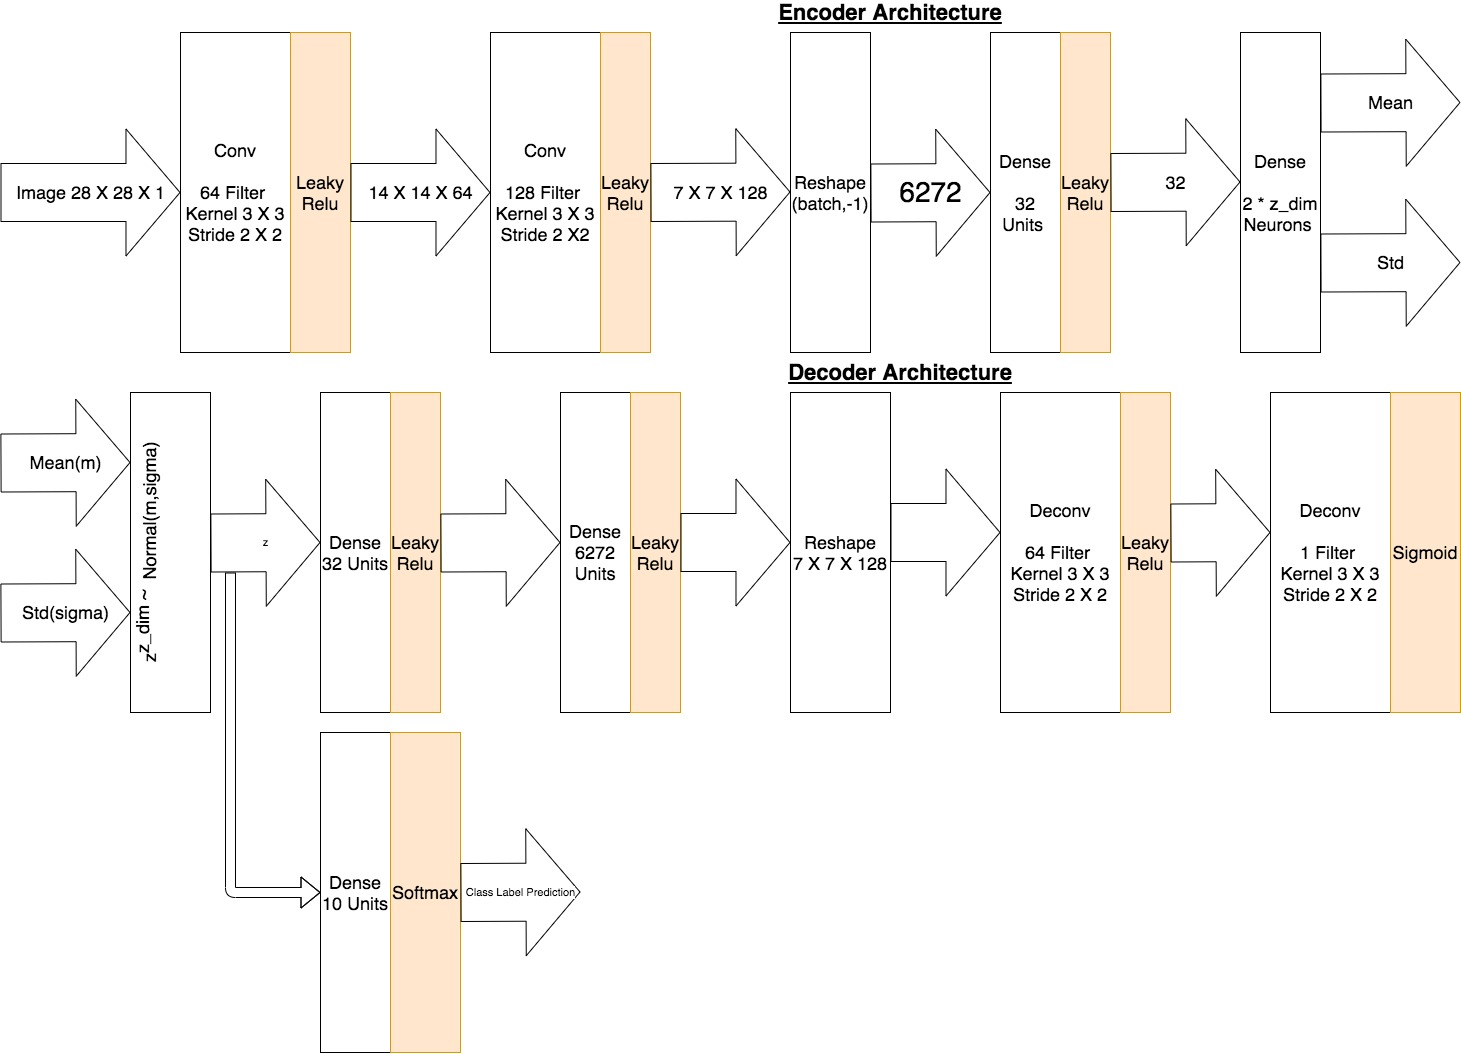
\includegraphics[width=3.5in]{vae_model_architecture_classification.jpg}
% where an .eps filename suffix will be assumed under latex,
% and a .pdf suffix will be assumed for pdflatex; or what has been declared
% via
\DeclareGraphicsExtensions.
\caption{Proposed model architecture}
\label{vae_architecture}
\end{figure}

\section{Results and Discussions} \label{results}

We trained the network for a total of 5 epochs in two different ways.
\begin{enumerate}
    \item Completely unsupervised using only the variational autoencoder loss function mentioned in equation \ref{vae_loss_eqn} for all 5 epochs.
    \item Using semi-supervised loss function mentioned in equation \ref{semi_supervised_loss} after first two epochs
\end{enumerate}


Figure\ref{reconstruction_accuracy} shows  the reconstruction accuracy of the variational autoencoder on the validation images after 5 epochs of training with $\gamma = 0$  plotted as a function of latent vector dimension $z_{dim}$.
It is observed that increasing $z_{dim}$ beyond 10 does not result in an increase in accuracy in the same proportion.
This is because the number of nodes in the 3rd layer were fixed at 32 which limits the representational capacity of that and all the subsequent layers.

We choose $z_{dim}=10$ to run the  semi-supervised model, experiment 2 mentioned above,  with both reconstruction and classification loss.
We ran semi-supervised experiment with different choices of clustering algorithms ( k-means and gmm) and using different confidence decay function.
Figure \ref{classification_accuracy_comparison} shows the classification accuracy on MNIST test images after 5 epochs with different choices of clustering and confidence function.
Figure\ref{cluster_center_1_gmm} shows the decoded cluster center images after the first epoch and Figure\ref{cluster_center_6_gmm} shows the cluster centers after 5 epochs of training using gmm clustering.
It is evident from this figure that as the training progresses the cluster centers get closer to the real semantic classes.


The model gave a classification accuracy of 93.47\% on test images within 5 epochs with only 10-16 images ( corresponding to each  cluster center) annotated after each epoch.
The labels given to the cluster center were propagated to all other samples in the cluster and this increases the effective number of labelled samples by a huge factor.

A comparison of reconstruction accuracy with and without classification loss added is shown in Figure \ref{reconstruction_accuracy_sup_vs_unsup}.
The blue curve in figure shows the reconstruction accuracy when the latent vectors were clustered and a label were assigned to the reconstructed images corresponding to  cluster centers at the end of every epoch.
The figure shows that the reconstruction accuracy of VAE is improved significantly  (by 6 to 10 \%) when classification loss is added, which indicates that the learned representation generalizes better as in the case of many multi-tasking models.

The distribution of data points were visualized by reducing the latent vector dimension from 10 to 2.
Fig \ref{tsne_unsup} shows the distribution with 5 epochs of unsupervised training i.e using only autoencoder loss.
Fig \ref{tsne_semi} shows the same for semi-supervised classification with gmm clustering.
From the distribution it is evident that
\begin{enumerate}
\item Semi-supervised learning generates semantically valid clusters
\item Clusters with semi-supervised learning are more separated as compared to the latent space learned by unsupervised auto-encoder
\end{enumerate}

\begin{figure}[]
\centering
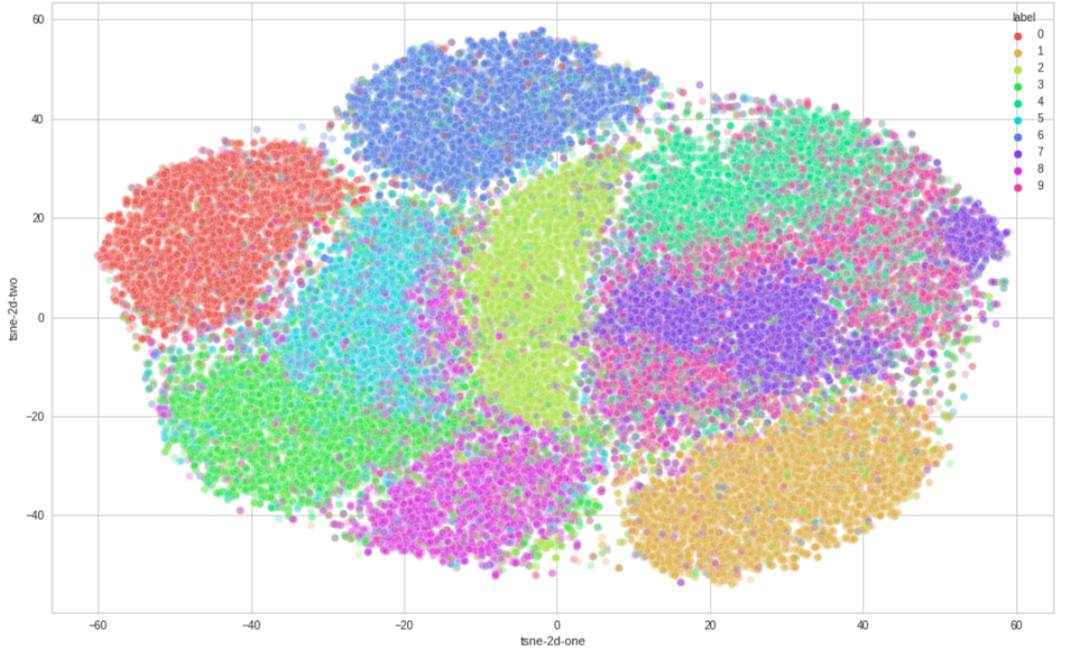
\includegraphics[width=\linewidth]{tsne_unsup}
\caption{2 dimensional tsne Visualization of latent space for MNIST imgaes obtained using unsupervised autoencoder }
\label{tsne_unsup}
\end{figure}

\begin{figure}[]
\centering
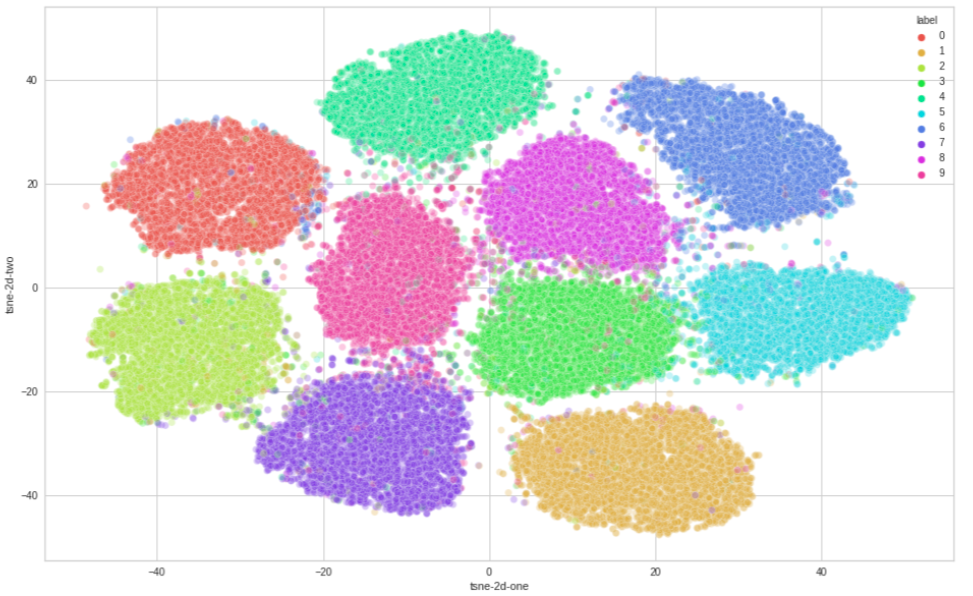
\includegraphics[width=\linewidth]{tsne_semi.png}
\caption{2 dimensional tsne Visualization of latent space for MNIST imgaes obtained using semisupervised training }
\label{tsne_semi}
\end{figure}

\begin{figure}[]
\centering
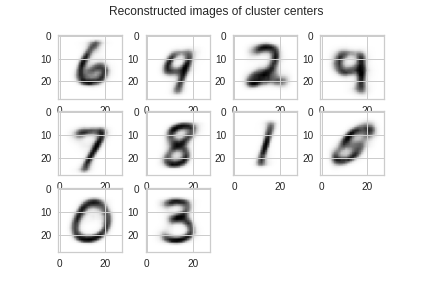
\includegraphics[width=\linewidth]{cluster_centers_epoch_1_0_gmm.png}
\caption{Images of decoded cluster center after first epoch}
\label{cluster_center_1_gmm}
\end{figure}

\begin{figure}[]
\centering
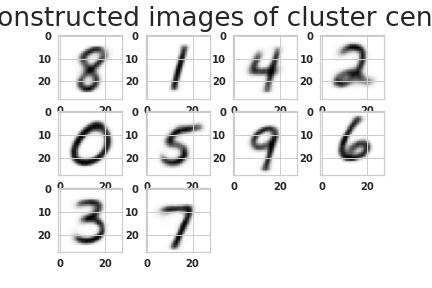
\includegraphics[width=\linewidth]{cluster_centers_epoch_5_0_gmm.png}
\caption{Images of decoded cluster center after 5th epoch}
\label{cluster_center_6_gmm}
\end{figure}

\begin{figure}[]
\centering
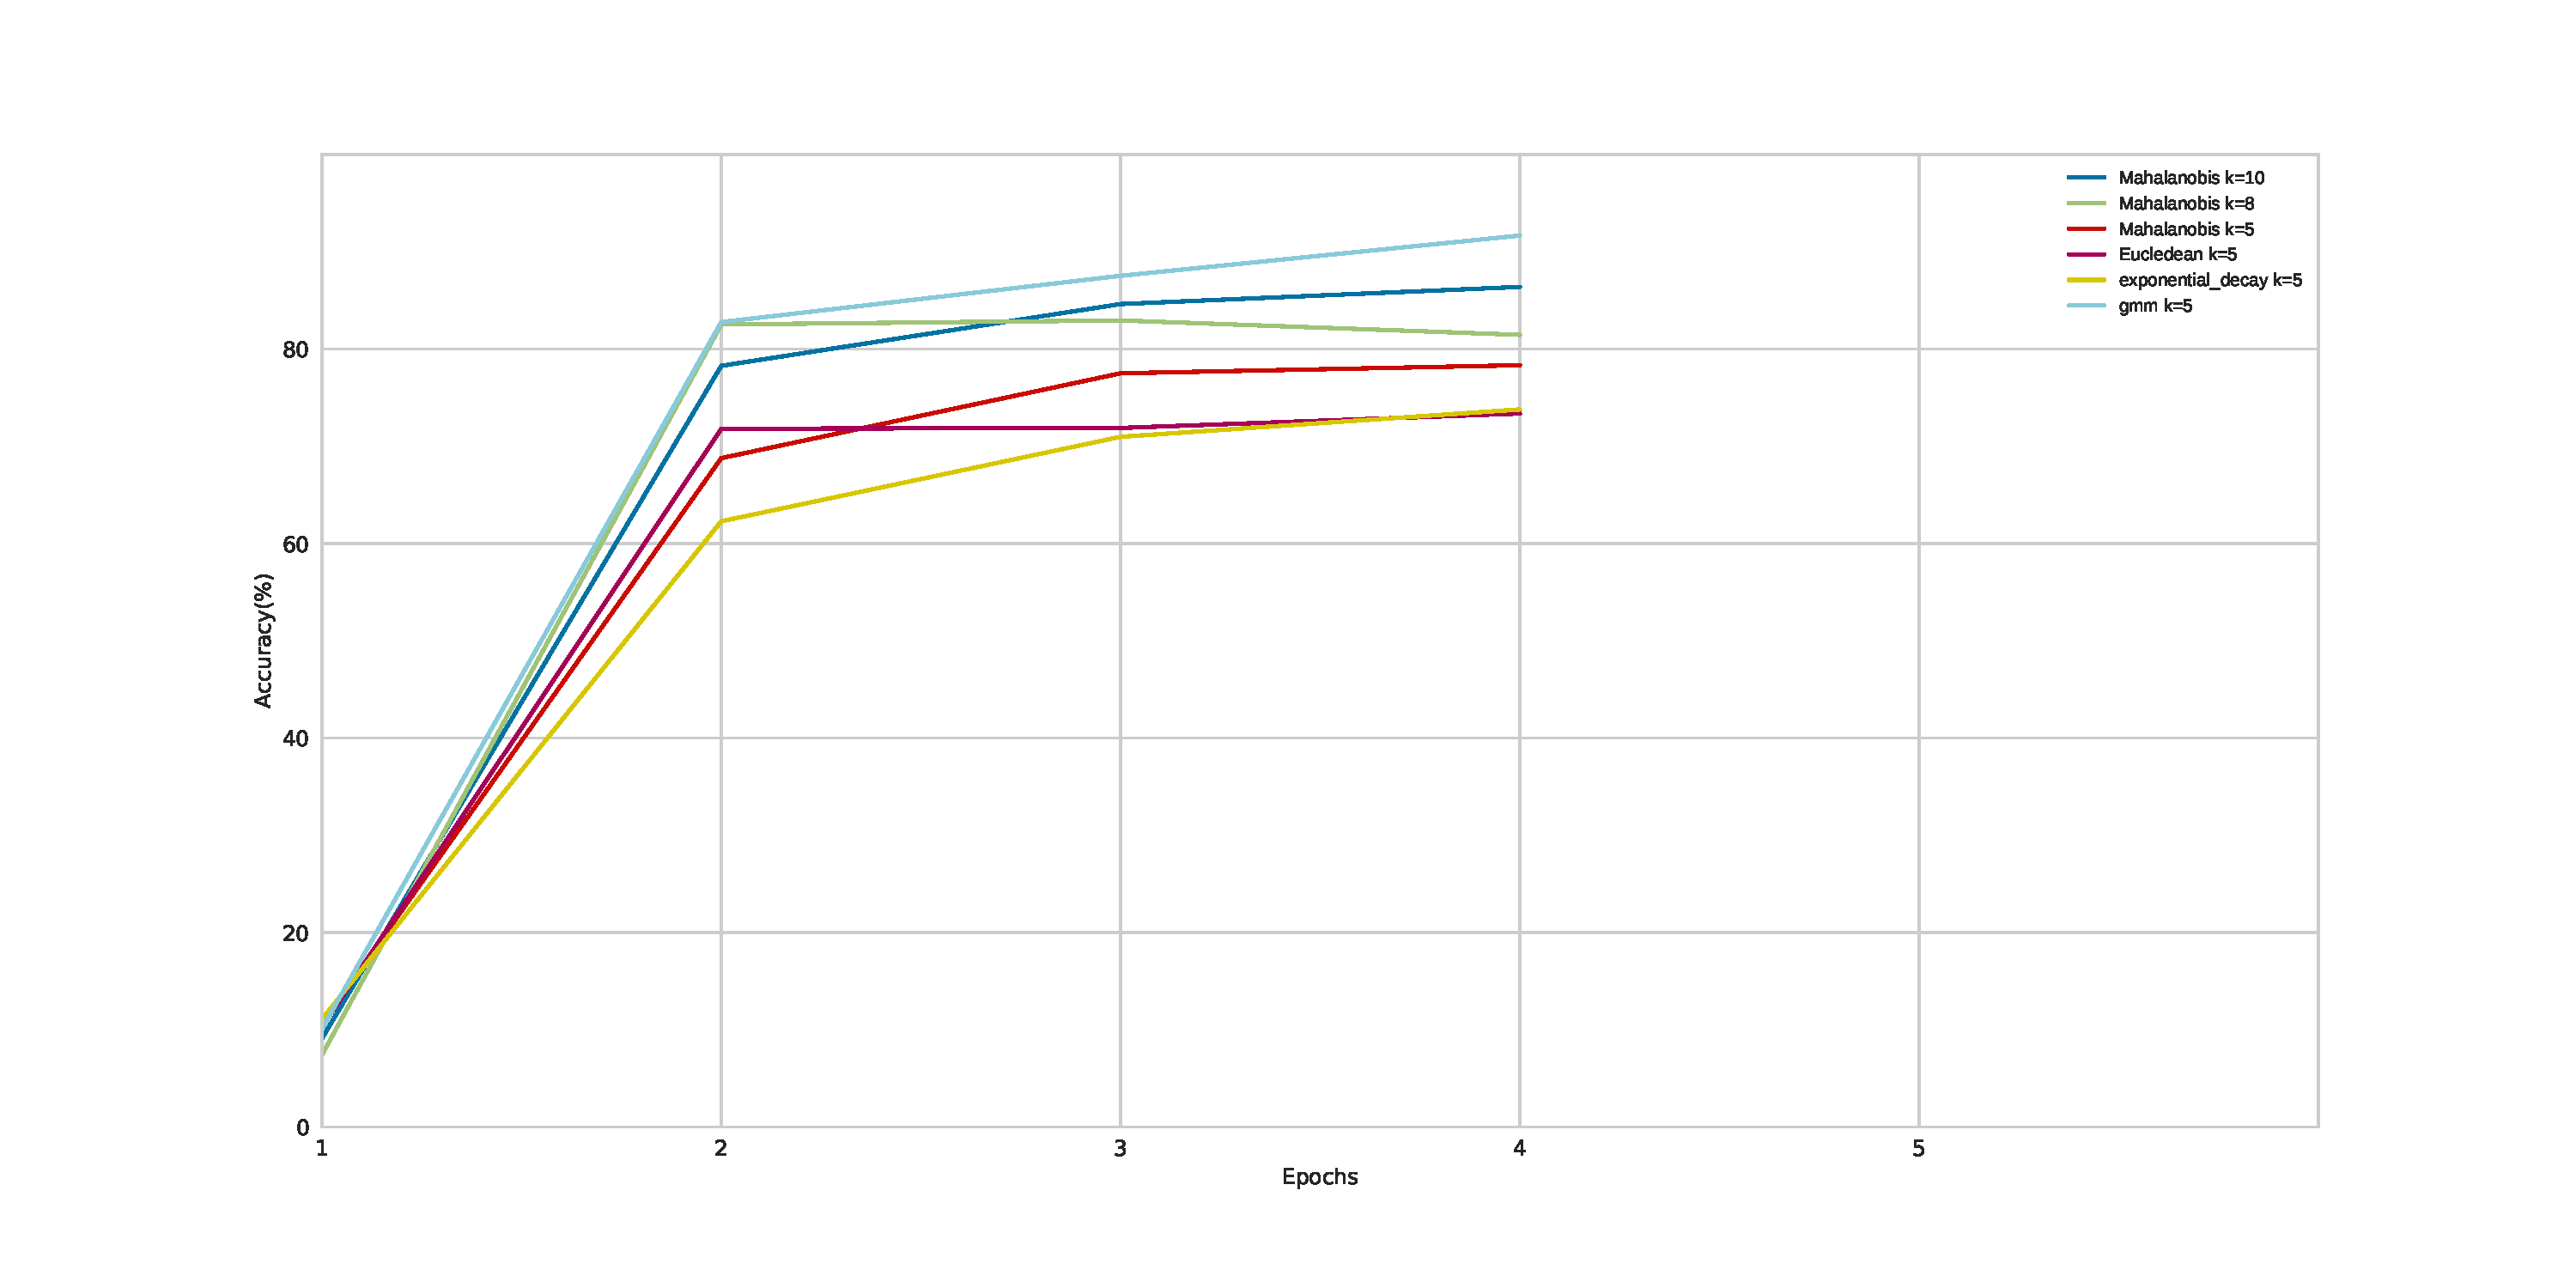
\includegraphics[width=\linewidth]{classification_accuracy_comparison}
\caption{Classification accuracy on test images using semi-supervised trained with $z_{dim}=10$ and $\gamma = 150$}
\label{classification_accuracy_comparison}
\end{figure}

\begin{figure}[]
\centering
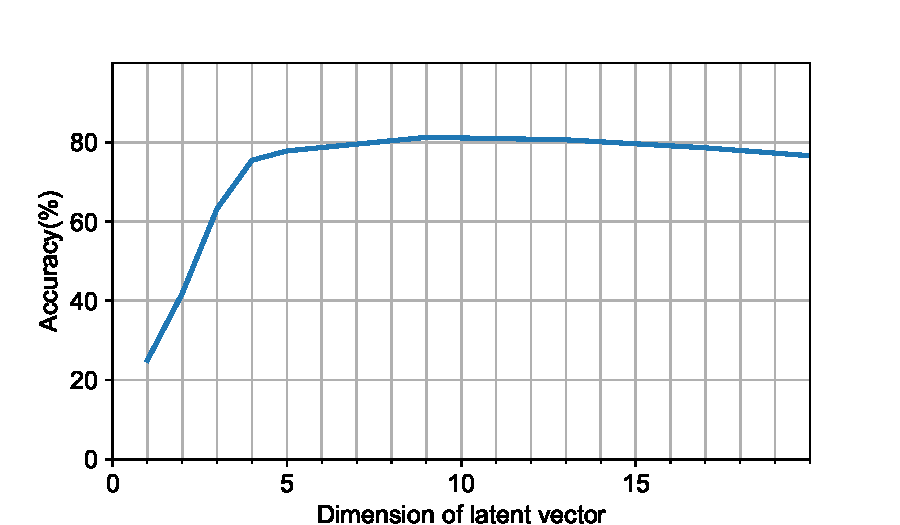
\includegraphics[width=\linewidth]{reconstruction_accuracy}
\caption{Reconstruction accuracy of autoencoder on validation images as a function the latent vector dimension  $z_{dim}$ and $\gamma = 0$}
\label{reconstruction_accuracy}
\end{figure}

\begin{figure}[!t]
\centering
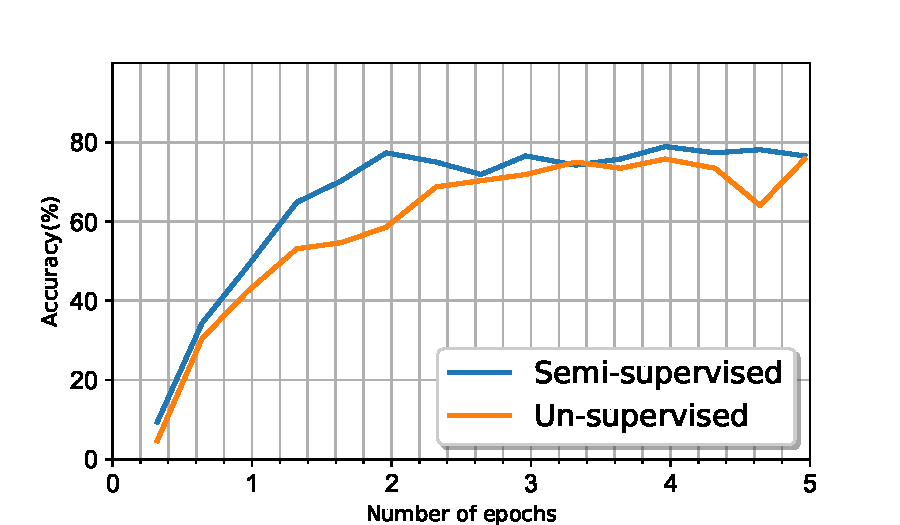
\includegraphics[width=\linewidth]{reconstruction_accuracy_different_runs}
\caption{Comparison of reconstruction accuracy with and without classification loss }
\label{reconstruction_accuracy_sup_vs_unsup}
\end{figure}

\section{Conclusion} \label{conclusion}
We propose a novel deep learning based active learning framework for solving complex tasks like image classification and segmentation.
The proposed approach is demonstrated by classifying MNIST images by annotating only 10-16 images, corresponding to each cluster center,  after each epoch.
We were able to obtain a classification accuracy of 93.47\% after 5 epochs of training.
It is possible to increase this accuracy further by increasing the number of clustering levels.
It is also observed that the reconstruction accuracy of the generative model improves as a result of performing an auxiliary task of classification
Another key observation of our study is that the formation of semantically valid clusters as a result of adding supervised loss and it is also observed that these clusters become more separable compared to the purely unsupervised counterpart
%\subsection{References, Citations, Footnotes}\label{sec:etc}
%\subsubsection{Cross-Referencing}
%Always use \verb|\label| and \verb|\ref|—or a command with a similar effect—when cross-referencing.
%For example, this subsection is Section~\ref{sec:etc}.
%
%\section{Floats}\label{sec:floats}
%Floats, such as figures, tables and algorithms, are moving objects and are supposed to float to the nearest convenient location.
%Please do not force them to go in the middle of a paragraph.
%They must respect the column width.
%
%Two-column floats are possible.
%They appear at the top of the next page, so strategic placement may be necessary.
%For an example, see Figure~\ref{fig:tikz}.
%They may not enter the margins.
%\begin{figure*}
%    \centering
%    \begin{tikzpicture}[xscale=1.5]
%        \coordinate (origin);
%        \draw[->] (origin) -- +(1cm,0) node[below] {$x$};
%        \draw[->] (origin) -- +(0,1cm) node[left] {$y$};
%        \fill[gray] (45:1cm) circle[radius=.2cm];
%    \end{tikzpicture}
%    \caption{A Nice Filled Ellipse with a Pair of Coordinate Axes.}\label{fig:tikz}
%\end{figure*}

%All material in floats should be legible and of good quality.
%So avoid very small or large text and pixelated or fuzzy lines.

%\subsection{Figures}\label{sec:figures}
%Figures should go in the \texttt{figure} environment and be centered therein.
%The caption should go below the figure.
%Use \verb|\includegraphics| for external graphics files but omit the file extension.
%Supported formats are \textsf{pdf} (preferred for vector drawings and diagrams), \textsf{png} (preferred for screenshots), and \textsf{jpeg} (preferred for photographs).
%Do not use \verb|\epsfig| or \verb|\psfig|.
%If you want to scale the image, it is better to use a fraction of the line width rather than an explicit length.
%For example, see Figure~\ref{fig:toronto}.
%\begin{figure}
%  \centering
%  \includegraphics[width=0.7\linewidth,page=3]{toronto}
%  \caption{A View of a Nice City.}\label{fig:toronto}
%\end{figure}
%
%Do not use \verb|\graphicspath|.
%If the images are contained in a subdirectory, specify this when you include the image, for example \verb|\includegraphics{figures/mypic}|.
%
%
%\subsection{Algorithms}\label{sec:algorithms}
%You can load your favorite algorithm package, such as \textsf{algorithm2e}\footnote{See the \textsf{algorithm2e} documentation at \url{https://ctan.org/pkg/algorithm2e}.}.
%Use the environment defined in the package to create a centered float with an algorithm inside.
%
%\section{Back Matter}
%There are a some final, special sections that come at the back of the paper, in the following order:
%\begin{itemize}
%  \item Author Contributions
%  \item Acknowledgements
%  \item References
%\end{itemize}
%They all use an unnumbered \verb|\subsubsection|.
%
%For the first two special environments are provided.
%(These sections are automatically removed for the anonymous submission version of your paper.)
%The third is the ‘References’ section.
%(See below.)
%
%(This ‘Back Matter’ section itself should not be included in your paper.)

\begin{contributions} % will be removed in pdf for initial submission,
                      % so you can already fill it to test with the
                      % ‘accepted’ class option
    Briefly list author contributions.
    This is a nice way of making clear who did what and to give proper credit.

    H.~Q.~Bovik conceived the idea and wrote the paper.
    Coauthor One created the code.
    Coauthor Two created the figures.
\end{contributions}

\begin{acknowledgements} % will be removed in pdf for initial submission,
                         % so you can already fill it to test with the
                         % ‘accepted’ class option
    Briefly acknowledge people and organizations here.

    \emph{All} acknowledgements go in this section.
\end{acknowledgements}

\bibliography{semi_supervised_learning}

\appendix
% NOTE: necessary when ptmx or no mathfont class option is given
%\providecommand{\upGamma}{\Gamma}
%\providecommand{\uppi}{\pi}
%\section{Math font exposition}
%How math looks in equations is important:
%\begin{equation*}
%  F_{\alpha,\beta}^\eta(z) = \upGamma(\tfrac{3}{2}) \prod_{\ell=1}^\infty\eta \frac{z^\ell}{\ell} + \frac{1}{2\uppi}\int_{-\infty}^z\alpha \sum_{k=1}^\infty x^{\beta k}\mathrm{d}x.
%\end{equation*}
%However, one should not ignore how well math mixes with text:
%The frobble function \(f\) transforms zabbies \(z\) into yannies \(y\).
%It is a polynomial \(f(z)=\alpha z + \beta z^2\), where \(-n<\alpha<\beta/n\leq\gamma\), with \(\gamma\) a positive real number.

\end{document}
